\documentclass[a4paper,10pt]{article}

\usepackage{amssymb}
\usepackage{amsmath}

\addtolength{\textwidth}{2.2cm}  
\addtolength{\oddsidemargin}{-1.10cm}
\addtolength{\evensidemargin}{-1.10cm}
\addtolength{\textheight}{2.0cm} 
\addtolength{\topmargin}{-1.2cm}

\usepackage{colortbl}

\usepackage{fancybox}
\usepackage{pgf}
\usepackage{tikz}
\usetikzlibrary{calc,shapes,snakes,arrows,shadows}


\begin{document}

\title{About the format of the B.out and B.iout files}

\author{Diego Fabregat-Traver}

\date{November, 2012}

\maketitle

The output from CLAK-GWAS is divided in two files: {\tt B.out} and {\tt B.iout}.
The first stores the actual data, the second the metadata.

\vspace{3mm}
\noindent
The metadata file format is as follows:

\begin{verbatim}
int type     // Double -> 6 as in Databel
int nbytes   // Double -> 8
int p        // # of covariates + 2 (intercept and SNP)
int m        // # of SNPs
int t        // # of traits
int tile_m   // More on these two later
int tile_t
int namelength // 32 as in Databel
char * labels  // More in a second
\end{verbatim}

\vspace{3mm}
\noindent
Labels:

\begin{itemize}
	\item Beta labels: {\tt beta\_intercept}, {\tt beta\_cov1}, ... , {\tt beta\_SNP}
	\item SE labels: {\tt se\_intercept}, {\tt se\_cov1}, ... , {\tt se\_SNP}
	\item Covariates labels: {\tt cov\_cov1\_intercept}, {\tt cov\_cov2\_intercept}, ... , {\tt cov\_SNP\_intercept}, {\tt cov\_cov2\_cov1}, ...
\end{itemize}

\vspace{3mm}
\noindent
Essentially, the labels are the betas, then the diagonal of the var-cov matrix, and then the lower triangle by columns.


\vspace{3mm}
\noindent
The data file ({\tt B.out}) is simply a long sequence of doubles. 
The way data is stored is a bit complicated if you are not used to this. Let me explain
based on the figure below.
The entire grid of results for $m$ SNPs $\times$ $t$ traits is stored in blocks or {\em tiles} of size
$tile_m \times tile_t$. Tiles are stored column-wise: First {\tt T0}, then {\tt T1} and so on.
Within each tile, data is also stored column-wise: (Trait0, SNP0), (Trait0, SNP1), (Trait0, SNP2), ..., (Trait0, SNP(m-1)), (Trait1, SNP0), ...

	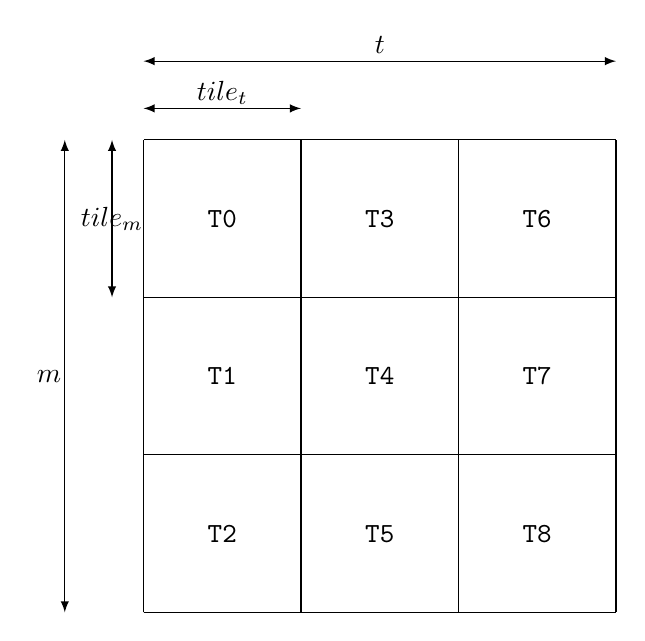
\begin{tikzpicture}

		\draw [ystep=2.0,xstep=2.0] (0,0) grid (6,6);

		\draw[black, latex-latex] ( 0, 7.0 ) -- ( 6, 7.0 );
		\draw[black, latex-latex] ( -1.0, 0 ) -- ( -1.0, 6 );
		\draw[black, latex-latex] ( 0, 6.4 ) -- ( 2, 6.4 );
		\draw[black, latex-latex] ( -0.4, 4 ) -- ( -0.4, 6 );
		\node[at={(3, 7.2)}] {$t$};
		\node[at={(-1.2, 3)}] {$m$};
		\node[at={(1, 6.6)}] {$tile_t$};
		\node[at={(-0.4, 5)}] {$tile_m$};

		\node[at={( 1, 5 )}] {\tt T0};
		\node[at={( 1, 3 )}] {\tt T1};
		\node[at={( 1, 1 )}] {\tt T2};
		\node[at={( 3, 5 )}] {\tt T3};
		\node[at={( 3, 3 )}] {\tt T4};
		\node[at={( 3, 1 )}] {\tt T5};
		\node[at={( 5, 5 )}] {\tt T6};
		\node[at={( 5, 3 )}] {\tt T7};
		\node[at={( 5, 1 )}] {\tt T8};
		
	\end{tikzpicture}

\vspace{15mm}
\noindent
Now, each entry (Trait*, SNP*) is actually an array containing all the values for the 
corresponding beta and lower triangle of the var-cov. For instance, if we have 2 covariates
(sex, age) and a SNP (rs33), with a var-cov matrix:

\vspace{5mm}
\begin{tabular}{| c | c  c  c  c |} \hline
	\# & Int & sex & age & rs33 \\\hline
	Int &  se\_Int & * & * & * \\
	sex &  cov\_sex\_Int & se\_sex & * & * \\
	age &  cov\_age\_Int & cov\_age\_sex & se\_age & * \\
	rs33 & cov\_rs33\_Int & cov\_rs33\_sex & cov\_rs33\_age & se\_rs33 \\\hline
\end{tabular}


\vspace{5mm}
\noindent
The array is as follows:

\begin{verbatim}
[beta_Int, beta_sex, beta_age, beta_rs33, se_Int, se_sex, se_age, se_rs33, 
 cov_sex_Int, cov_age_Int, cov_rs33_Int, cov_age_sex, cov_rs33_sex, cov_rs33_age]
\end{verbatim}

\vspace{1mm}
\noindent
Notice that the order matches the one for the labels in the file {\tt B.iout}.


\vspace{5mm}
\noindent
All the data above occupies $m \times t \times (p + p*(p+1)/2)$ doubles. After all these values,
you can find the estimates: heritability, sigma, res\_sigma, and beta estimates, 
for a total of $(3 + (p-1)) \times t$ values. The storage is the following: 
first the $t$ heritability values (again trait0, trait1, ..., trait(t-1));
then the $t$ sigmas; then $t$ res\_sigmas; and finally the $t$ beta estimates.
The beta estimates are stored as expected: beta\_Int, beta\_cov1, ..., beta\_cov(p-2).

\end{document}
